% Created 2015-06-22 Mon 16:43
\documentclass[10pt]{article}
\usepackage[utf8]{inputenc}
\usepackage[T1]{fontenc}
\usepackage{fixltx2e}
\usepackage{graphicx}
\usepackage{longtable}
\usepackage{float}
\usepackage{wrapfig}
\usepackage{rotating}
\usepackage[normalem]{ulem}
\usepackage{amsmath}
\usepackage{textcomp}
\usepackage{marvosym}
\usepackage{wasysym}
\usepackage{amssymb}
\usepackage{hyperref}
\tolerance=1000
\usepackage{a4wide}
\usepackage{todonotes}
\setcounter{secnumdepth}{3}
\author{Quang - Vinh DANG}
\date{\today}
\title{Reproducibility Notebook for 'Performance evaluation of Google Docs'}
\hypersetup{
  pdfkeywords={},
  pdfsubject={},
  pdfcreator={Emacs 24.4.1 (Org mode 8.2.10)}}
\begin{document}

\maketitle
\tableofcontents

\makeatletter
\renewcommand{\verbatim@font}{\ttfamily\footnotesize}
\makeatother


\section{Project Overview}
\label{sec-1}

\subsection{Purpose of the experiment}
\label{sec-1-1}
Perform the evaluation of Google Docs's performance in collaborative editing large scale settings.


\section{Data Analysis}
\label{sec-2}

\subsection{Setup}
\label{sec-2-1}

\begin{itemize}
\item It is suggested that the measurement should be run on multiple computers that are accessible between each others. However, running on a single computer is possible.

\item If the users decide to run the measurement on multiple computers, there are several small steps need to be done manually. These steps are not required in case running on a single computer.

\item The next steps are:

\begin{itemize}
\item We need 1 master computer, where the measurement will run on and controls other computers.
\item For each other slave computers:

\begin{itemize}
\item Download chromedriver at sites.google.com/a/chromium.org/chromedriver/ and Selenium Standalone Server at www.seleniumhq.org/download. Unzip and put them in a same directory. Set the execute mod if needed (in *nix system). Then start selenium server as running an usual JAR file (java -jar selenium-server-jar-file) inside the directory which contains these files.
\end{itemize}

\item On the master computer, download, unzip and put chromedriver into the same directory with this document. The chromedriver for Linux has been already provided. Set the execute mode for chromedriver file also.

\item On the master computer, open the file "selenium\_config.txt" provided with this document.

\begin{itemize}
\item The first line (LOCAL) decides how many clients you want to simulate in the master computer. If you run with a single master computer and no slave, the number follows the keyword "LOCAL" should be 50. The recommend value is 0.

\item The following lines are IP address or hostnames if possible of each slave computers and the number of clients you want to simulate for each slave computers, one for a line.

\item The last line is the IP address or hostname of one slave computer, which will handle all other requests in the case the number of requests in runtime exceed the total number you defined both master computer and slave computers in above lines. For instance, if you defined that the master computer will simulate up to 10 clients and the slave computer number 1 (you have only 1 slave computer) will simulate 20 clients, but in runtime you requested the 31st client - this client will be simulated by the machine with IP address in the last line.
\end{itemize}

\item On the master computer, open the file "num\_user\_setting.txt" provided with this document.

\begin{itemize}
\item This file contains only one line, which defines what number of users we will run on measurement. For instance, if the line content is (without quotes) "1 5 10 20", the measurement will run first with 1 client, then 5 clients, and so on. You can modify this file if needed, otherwise leave it default. Please note that each numbers in the line are separated by space.
\end{itemize}

\item The file "last\_exp\_info.txt" provided with this document is handled automatically by the measurement. However, you can modify this file to skip or redo some particular measurement setting. The file contains the last experiment information, so if because of some reasons the measurement stops, next time it will start by its last experiment but not run everything from beginning.
\end{itemize}

\item All computer requires Java SE to be installed. The measurement has been developed with JDK 8 so it is the recommend version. Google Chrome browsers also need to be updated to the latest version. To process data after the measurement finished, Python 2.7+ and R (version 3.2.1 or later) are required.
\end{itemize}
\subsection{Running the experiment}
\label{sec-2-2}

\begin{verbatim}
java -jar GoogleDocs.jar
\end{verbatim}

\subsection{Data processing}
\label{sec-2-3}

\subsubsection{The result as raw data will be provided in file "googledocs.txt".}
\label{sec-2-3-1}
\subsubsection{We provided a Python script to parse this data}
\label{sec-2-3-2}

\begin{verbatim}
python processResult.py googledocs.txt googledocs-delays.txt
\end{verbatim}

\subsection{Delay Visualization}
\label{sec-2-4}

\begin{verbatim}
#source ("ProcessData.R")
try_regression <- function (file_name, speed=1, poly = 3, x_step=2)
{
  #setwd ("/Users/qdang/workspace/collborative_editing_measurement")
  plot.new()
  df <- read.table (file_name, header = TRUE)
  df$delay <- df$delay / 1000
  df <- df [df$speed == speed,]
  means <- tapply (df$delay, df$user, mean)
  lm <- lm (means ~ poly (unique(df$user), 3))
  boxplot (df$delay ~ df$user,ylab="Delay in seconds", xlab="Number of user", 
	   main=paste("Google Docs performance with typing speed = ", speed, " char/sec"), las=2)
  #axis(side=1,at=seq(0,50,by=x_step),las=2)
  #lines (unique (df$user), predict (lm), col="red")
  lines (predict(lm), col = "red")
  lm
}

processAllGoogleDocs <- function (file_name, poly = 3, x_step = 2) {
  df <- read.table (file_name, header = TRUE)   #read data
  df$delay <- df$delay / 1000 #convert to seconds
  speeds <- c (1,2,4,5,6,8, 10)
  for (speed in speeds) {
    model = try_regression (file_name = file_name, speed = speed, poly = poly, x_step = x_step)
    summary(model)
  }
}
#processAllGoogleDocs ("googledocs-delays.txt")
model1 = try_regression("googledocs-delays.txt", speed = 1)
\end{verbatim}

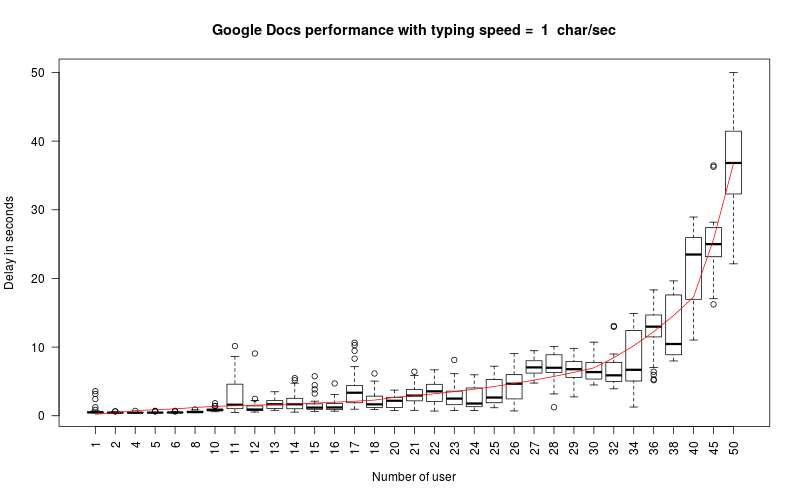
\includegraphics[width=.9\linewidth]{figs/g1.png}

\begin{verbatim}
summary (model1)
\end{verbatim}

\begin{verbatim}
Call:
lm(formula = means ~ poly(unique(df$user), 3))

Residuals:
    Min      1Q  Median      3Q     Max 
-2.0590 -0.4989 -0.2889  0.2166  4.5543 

Coefficients:
                          Estimate Std. Error t value Pr(>|t|)    
(Intercept)                 5.9085     0.2226  26.541  < 2e-16 ***
poly(unique(df$user), 3)1  37.7039     1.2789  29.483  < 2e-16 ***
poly(unique(df$user), 3)2  22.3560     1.2789  17.481  < 2e-16 ***
poly(unique(df$user), 3)3   6.8780     1.2789   5.378 8.87e-06 ***
---
Signif. codes:  0 ‘***’ 0.001 ‘**’ 0.01 ‘*’ 0.05 ‘.’ 0.1 ‘ ’ 1

Residual standard error: 1.279 on 29 degrees of freedom
Multiple R-squared:  0.9765,	Adjusted R-squared:  0.974 
F-statistic: 401.2 on 3 and 29 DF,  p-value: < 2.2e-16
\end{verbatim}

\begin{verbatim}
model2 = try_regression ("googledocs-delays.txt", speed = 2)
\end{verbatim}

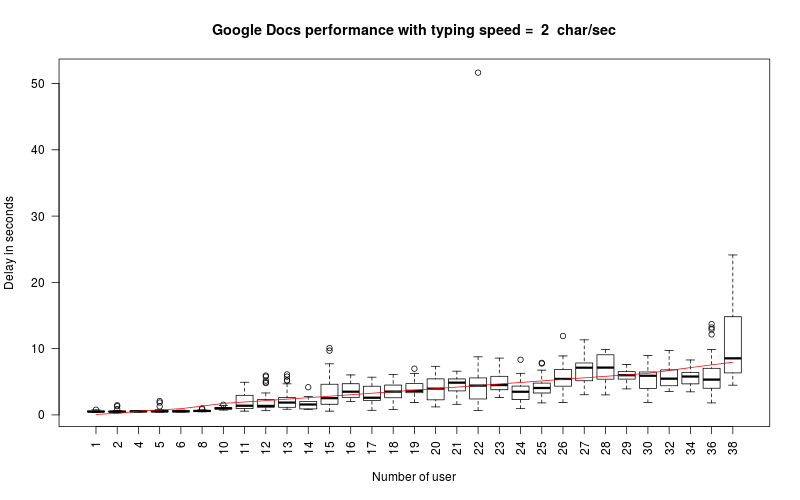
\includegraphics[width=.9\linewidth]{figs/g2.png}

\begin{verbatim}
summary (model2)
\end{verbatim}

\begin{verbatim}
Call:
lm(formula = means ~ poly(unique(df$user), 3))

Residuals:
     Min       1Q   Median       3Q      Max 
-1.43609 -0.63532  0.01539  0.35220  2.17281 

Coefficients:
                          Estimate Std. Error t value Pr(>|t|)    
(Intercept)                 3.7686     0.1601  23.540  < 2e-16 ***
poly(unique(df$user), 3)1  12.3366     0.8913  13.840 8.87e-14 ***
poly(unique(df$user), 3)2   0.2992     0.8913   0.336    0.740    
poly(unique(df$user), 3)3  -0.3266     0.8913  -0.366    0.717    
---
Signif. codes:  0 ‘***’ 0.001 ‘**’ 0.01 ‘*’ 0.05 ‘.’ 0.1 ‘ ’ 1

Residual standard error: 0.8913 on 27 degrees of freedom
Multiple R-squared:  0.8766,	Adjusted R-squared:  0.8629 
F-statistic: 63.94 on 3 and 27 DF,  p-value: 2.165e-12
\end{verbatim}

\begin{verbatim}
model4 = try_regression ("googledocs-delays.txt", speed = 4)
\end{verbatim}

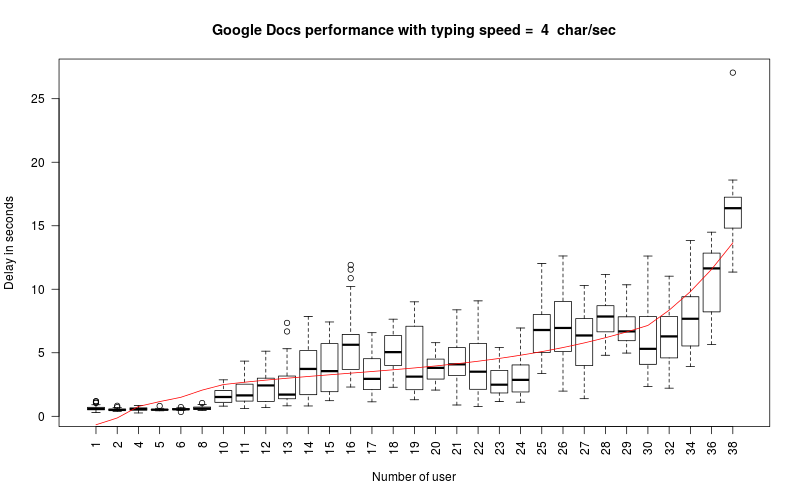
\includegraphics[width=.9\linewidth]{figs/g4.png}

\begin{verbatim}
summary (model4)
\end{verbatim}

\begin{verbatim}
Call:
lm(formula = means ~ poly(unique(df$user), 3))

Residuals:
    Min      1Q  Median      3Q     Max 
-2.3012 -0.9203 -0.1988  0.7029  2.8093 

Coefficients:
                          Estimate Std. Error t value Pr(>|t|)    
(Intercept)                 4.4495     0.2475  17.976  < 2e-16 ***
poly(unique(df$user), 3)1  16.3891     1.3782  11.892 3.05e-12 ***
poly(unique(df$user), 3)2   4.2534     1.3782   3.086  0.00464 ** 
poly(unique(df$user), 3)3   3.8992     1.3782   2.829  0.00869 ** 
---
Signif. codes:  0 ‘***’ 0.001 ‘**’ 0.01 ‘*’ 0.05 ‘.’ 0.1 ‘ ’ 1

Residual standard error: 1.378 on 27 degrees of freedom
Multiple R-squared:  0.8548,	Adjusted R-squared:  0.8387 
F-statistic: 52.98 on 3 and 27 DF,  p-value: 1.925e-11
\end{verbatim}

\begin{verbatim}
model6 = try_regression ("googledocs-delays.txt", speed = 6)
\end{verbatim}

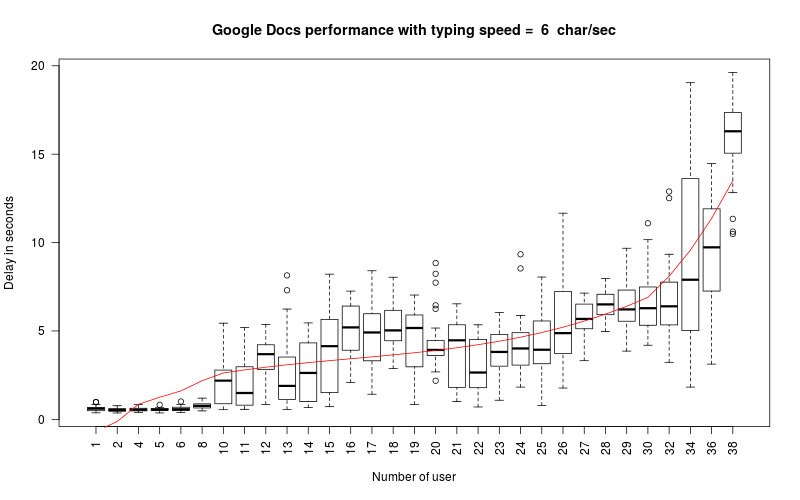
\includegraphics[width=.9\linewidth]{figs/g6.png}

\begin{verbatim}
summary (model6)
\end{verbatim}

\begin{verbatim}
Call:
lm(formula = means ~ poly(unique(df$user), 3))

Residuals:
    Min      1Q  Median      3Q     Max 
-1.8624 -0.6167 -0.2819  0.6203  2.3133 

Coefficients:
                          Estimate Std. Error t value Pr(>|t|)    
(Intercept)                 4.3929     0.1853  23.701  < 2e-16 ***
poly(unique(df$user), 3)1  15.7425     1.0320  15.255 8.55e-15 ***
poly(unique(df$user), 3)2   4.1655     1.0320   4.036 0.000402 ***
poly(unique(df$user), 3)3   4.2643     1.0320   4.132 0.000312 ***
---
Signif. codes:  0 ‘***’ 0.001 ‘**’ 0.01 ‘*’ 0.05 ‘.’ 0.1 ‘ ’ 1

Residual standard error: 1.032 on 27 degrees of freedom
Multiple R-squared:  0.9079,	Adjusted R-squared:  0.8976 
F-statistic: 88.69 on 3 and 27 DF,  p-value: 4.256e-14
\end{verbatim}

\begin{verbatim}
model8 = try_regression ("googledocs-delays.txt", speed = 8)
\end{verbatim}

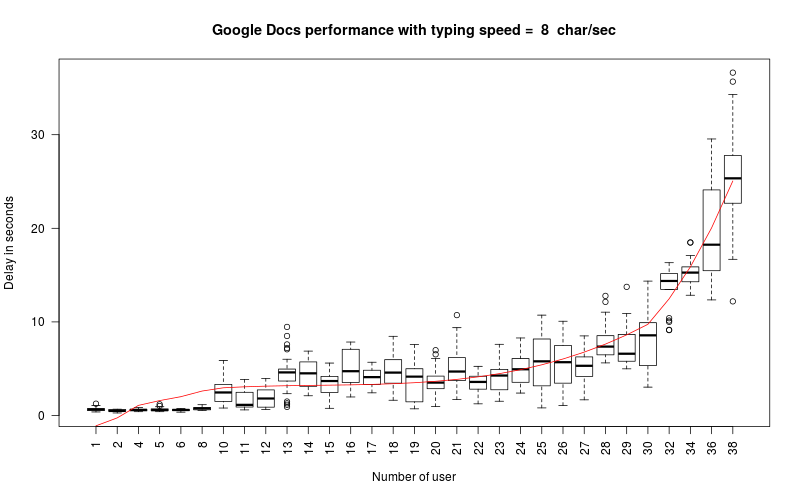
\includegraphics[width=.9\linewidth]{figs/g8.png}

\begin{verbatim}
summary (model8)
\end{verbatim}

\begin{verbatim}
Call:
lm(formula = means ~ poly(unique(df$user), 3))

Residuals:
     Min       1Q   Median       3Q      Max 
-1.85606 -0.79908  0.03254  0.85653  1.86847 

Coefficients:
                          Estimate Std. Error t value Pr(>|t|)    
(Intercept)                 5.7078     0.2048  27.870  < 2e-16 ***
poly(unique(df$user), 3)1  26.3486     1.1403  23.108  < 2e-16 ***
poly(unique(df$user), 3)2  13.8855     1.1403  12.177 1.77e-12 ***
poly(unique(df$user), 3)3   9.4437     1.1403   8.282 6.86e-09 ***
---
Signif. codes:  0 ‘***’ 0.001 ‘**’ 0.01 ‘*’ 0.05 ‘.’ 0.1 ‘ ’ 1

Residual standard error: 1.14 on 27 degrees of freedom
Multiple R-squared:  0.9653,	Adjusted R-squared:  0.9614 
F-statistic: 250.3 on 3 and 27 DF,  p-value: < 2.2e-16
\end{verbatim}

\begin{verbatim}
model10 = try_regression ("googledocs-delays.txt", speed = 10)
\end{verbatim}

\begin{verbatim}
summary (model10)
\end{verbatim}

\begin{verbatim}
Call:
lm(formula = means ~ poly(unique(df$user), 3))

Residuals:
    Min      1Q  Median      3Q     Max 
-4.9781 -1.5643  0.4321  1.3192  6.2262 

Coefficients:
                          Estimate Std. Error t value Pr(>|t|)    
(Intercept)                 5.7163     0.4043  14.140 5.33e-14 ***
poly(unique(df$user), 3)1  31.5617     2.2509  14.022 6.51e-14 ***
poly(unique(df$user), 3)2  21.6410     2.2509   9.614 3.28e-10 ***
poly(unique(df$user), 3)3  15.2678     2.2509   6.783 2.77e-07 ***
---
Signif. codes:  0 ‘***’ 0.001 ‘**’ 0.01 ‘*’ 0.05 ‘.’ 0.1 ‘ ’ 1

Residual standard error: 2.251 on 27 degrees of freedom
Multiple R-squared:  0.9254,	Adjusted R-squared:  0.9171 
F-statistic: 111.7 on 3 and 27 DF,  p-value: 2.475e-15
\end{verbatim}
% Emacs 24.4.1 (Org mode 8.2.10)
\end{document}
